
In this chapter we will try to relate the sections to the conceptual managers in the game engine. The reason for doing this is to easier identify and describe the different responsibilites the game engine has:
\begin{itemize}
	\item \textbf{Question flow manager}: adapts the questions to the knowledge level of the student, and is flexible such that the student can choose his own path through the completion of each difficulty level. 
	\item \textbf{Conversation manager:} puts the questions with belonging answer elements in a sequence such that they fit to a scenario, using the workflow model. The conversation manager produces questions and answer keys from a template, in which the entity model is used to fill in data for the place holders in the template.
	\item \textbf{User manager:} keeps track of the user's skill, based on the performance on previous quizzes. It holds track of the scores on the current quiz, and it measures the user's progression.
\end{itemize}


\section{Question Flow Manager}

% -----------------------------------------------------------------------------------------------


As each question in a quiz are related to a certain component in the treatment plan or theme in the learning map, the student will be measured how well he performs on each of these themes. For the asthma guideline \parencite{RepublicofKeny2016}, we have identified four themes. Assessment where the student will be tested in the initial examination. Diagnosis, where the student will determine a diagnosis as well as the severity. Management, where the student will determine which actions should be done to treat and best give the best care to the patient. The last discipline is the follow-up, where the student will be tested in evaluating the treatment, give advise to and educate patient and caregivers, provide the right medication and regular follow-up.

By splitting up the score in themes, the student can easily see which areas he is strong and where he needs more training. 



We can also adapt the questions in each discipline to the student's level. If the student has proven to be very good in providing the right amount of medicine to asthma patient, we can provide more difficult questions to challenge the student some more. If he struggles at setting the right diagnose, we can provide more basic questions to strengthen the students basic knowledge. 




The student will also be provided with a total score, which will be the aggregated score of each of the disciplines. The student can compare the total score of e.g. the asthma quiz and the jaundice quiz, and see which medical condition he needs to train more on.



\subsection{Dynamic Content Management}
The game engine is based on some of the concepts presented in the articles of \textcite{Eide2008}, \textcite{Kristensen2011} and \textcite{Kristensen2013}. The motivation for using DCM, is to support the principles of adaptive learning as well as flexibility in the learning process. Adaptive learning means that the student can solve problems which are suited to his knowledge level. Flexibility in the sense that the student can go through the learning content in many different ways.

\textcite{Eide2008} presents a dynamic content management system (DCM) made for e-learning. In DCM the focus is on removing the tight coupling between the learning material and the teaching course. By analysing the learning material and course, they can define conceptual atomic units of knowledge which they put into a knowledge repository. From this repository they may draw knowledge elements and organize into the hierarchy of a course. To model a course they use concept maps, which are directed graphs, where the vertices are concept labels and edges indicates the relationships between vertices. DCM operates with three concept maps: knowledge map, learning map and student map. The knowledge map is used to model the entire content of the knowledge repository and the hierarchy structure of a course. A learning map is used to model a specific course and is a representation of the learning process. The content units (vertices) in the knowledge map gets expanded, and becomes evaluation and resource vertices in the learning map. Content units from the knowledge map can be omitted if they are not needed in the specific course. Detailed prerequisites can be specified for the content units. The student map represents the progress of a specific student taking a specific course. The edges shows which resources he has used, the evaluations of the student and in which order. 


When we apply this to our project, we will first decouple the content from the flow-chart of the paediatric possible asthma guideline \parencite{RepublicofKeny2016}. To decouple the flow-chart, we use the workflow model as a helping tool, ordering on how they should learn the clinical guideline. In figure \ref{fig:KnowledgeMap} we have identified knowledge elements and hierarchically structured the knowledge repository into a knowledge map. The edges shows the dependencies in the learning process. To learn how to evaluate a treatment and act accordingly to the evaluation, the student needs to know something about how to set a diagnosis and how to initially treat it. Hence there is an edge between follow-up and the other knowledge units.

\begin{figure}[h!]
	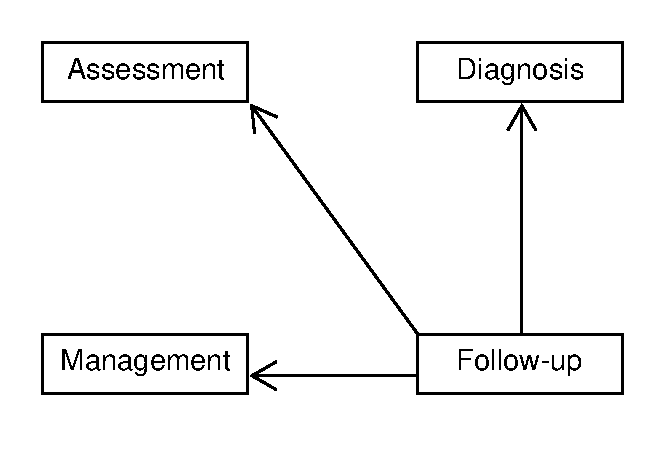
\includegraphics[scale=0.6]{KnowledgeMap3}
	\caption {Knowledge map}
	\label{fig:KnowledgeMap}
\end{figure}

In table \ref{table:ContentUnit} we have chosen a knowledge element from the knowledge map, and defined a content unit. The content unit contains a theme "Assessment". Resources is the learning material, which are relevant sections of the guideline. Evaluations are the tests to see if the student has reached the learning goals. At level 1 we try to learn facts about the guideline. In level 2 and 3 we give the student scenarios to work with.

\begin{table}[h!]
	\begin{tabular}{ | m{14em} | m{9em}| m{5em} | } 
		\hline
		\multicolumn{3}{c}{\bfseries T1: Assessment} \\
		\hline
		Resources & Evaluations & Aspects \\
		\hline
		R1: History and examination sections in the possible asthma guideline \parencite{RepublicofKeny2016} & E1: Quiz Level 1 & Facts \\
		& E2: Quiz Level 2 & Scenario \\
		& E3: Quiz Level 3 & Scenario \\
		\hline
	\end{tabular}
	\caption{The content unit Assessment}
	\label{table:ContentUnit}
\end{table}

In figure \ref{fig:LearningMap} we have identified four content units T1: Assessment, T2: Diagnosis, T3: Management and T4: Follow-up from the knowledge map. The importance of these content units in the asthma guideline \parencite{RepublicofKeny2016} was the reason these four got selected. The hierarchically structure of the knowledge map, makes the child nodes of the content units become learning material for their parent nodes.

Inside the content units in the learning map, we see the relationships between resources and evaluation. There is also dependencies between the content units. To be able to do a follow-up, a student needs to learn the assessment, diagnosis and management first, because follow-up is an evaluation and reaction to how the patient responded to the previous steps.  We have also specified the prerequisites for each evaluation. The prerequisites are written as logical expressions, as seven edges and operators per content unit would be confusing to read. What the prerequisites says is that all level 1 evaluations need to be completed before any level 2 evaluation can be taken. All level 2 evaluations need to be completed before any level 3 evaluation can be taken.

\begin{figure}[h!]
	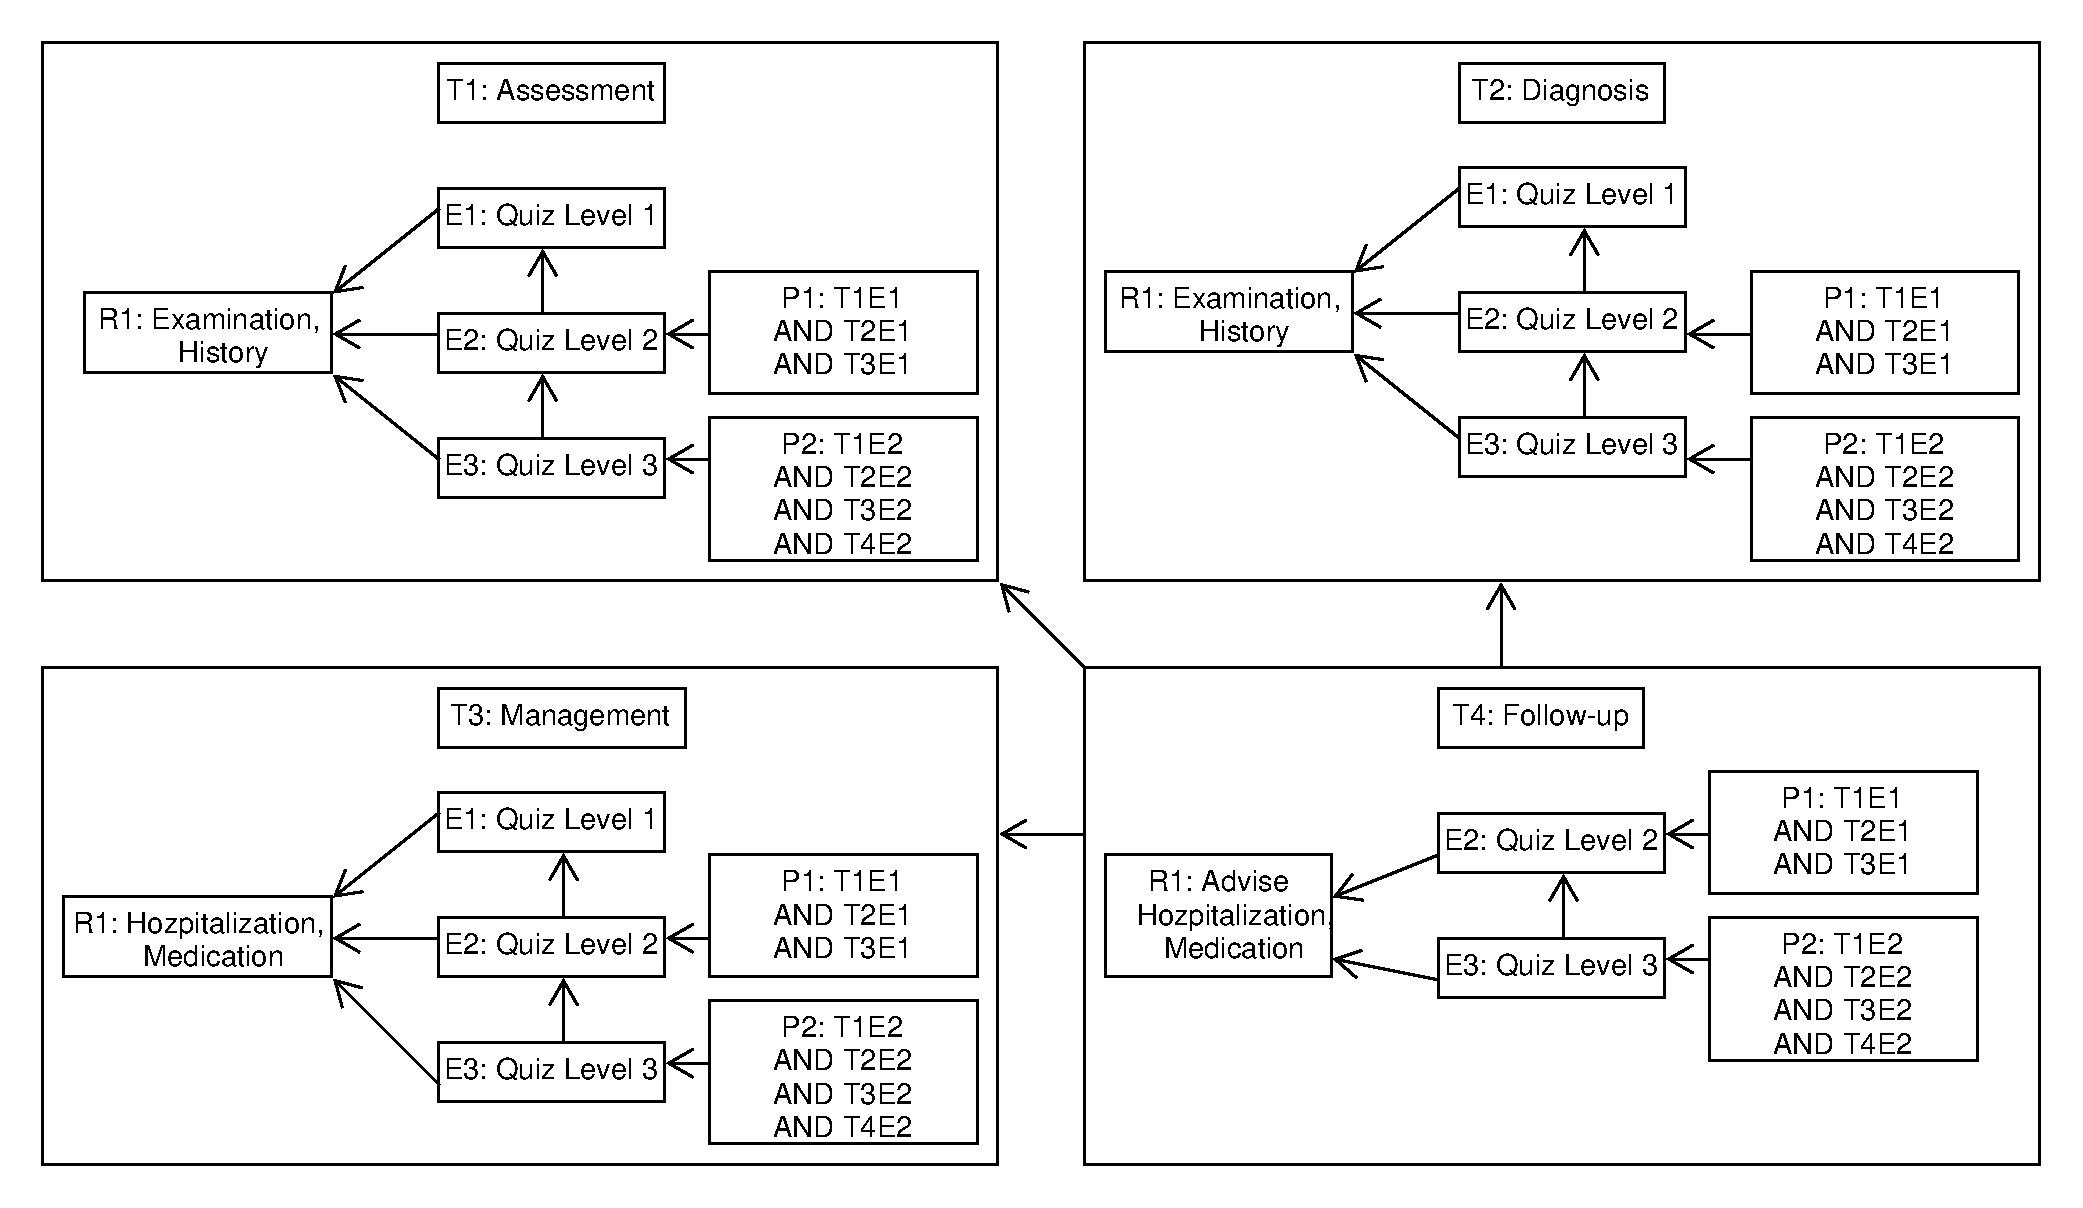
\includegraphics[scale=0.38]{LearningMap}
	\caption {Learning map}
	\label{fig:LearningMap}
\end{figure}

A student map would show the progressions for one specific student, and the path he has taken and the scores for each evaluation. Table \ref{table:StudentMap} shows a student's student map for the Assessment part of the course. He got the score 34 on the first evaluation. 34 matches the passing condition for assessment level 1, so he got a passing grade for that test. However, he scored 43 points on evaluation 2 and didn't meet the passing condition for that test. He has no attempts for evaluation 3, as he doesn't meet the prerequisites for that test.  The tests which have been completed are stored in the database on the students phone. In that sense, the database shows the student's current position in the learning map.

\begin{table}[h!]
	\begin{tabular}{ | m{12em} | m{8em}| m{5em} | } 
		\hline
		\multicolumn{3}{c}{\bfseries T1: Assessment} \\
		\hline
		Resources & Evaluations & Passed \\
		\hline
		R1: History and examination guideline & E1: 35 & True \\
		& E2: 43 & False \\
		& E3: &  \\
		\hline
	\end{tabular}
	\caption{Student Map T1:Assessment}
	\label{table:StudentMap}
\end{table}

\subsection{Types of questions}
We can further identify which kind of questions we are going to ask, by further examining the entity model and the workflow model combined. When we are doing an assessment in the workflow model, we are looking at the examination and history vertices of the entity graph. History is what the patient or the patient's dependent can tell around the patient's condition. Such that he has been coughing a lot the last days. Examination and history will provide the clinician with an idea of a diagnosis.

Diagnosis in the workflow model is connected to the history, examination and investigation. The clinician will continue asking questions, do examinations and probably order some tests to strengthen his assumption of the diagnosis. The clinician can also set a more specific diagnosis, such as in the asthma guideline \parencite{RepublicofKeny2016}, where we categorize in severe, mild and moderate asthma.

Management is how we manage the patient with the given diagnosis. Hospitalization is if we are going to set patient status to inpatient or outpatient. Medication is given to treat the patient or relieve the symptoms. Surgery is not part of the asthma guideline \parencite{RepublicofKeny2016}, but it is important to be aware that management procedures needs to be added when making quizzes for other conditions than asthma.

Follow-up will contain questions related how to evaluate the treatment and how to act upon the evaluation. The symptoms of the patient may have worsen, getting better or are unchanged after the treatment, and the clinician needs to act accordingly. The treatment may have been given at the hospital or it may have been something the patient have had to do at home. The patient may also get some instructions from the clinician when there is something he should do on his own.

\begin{figure}[h!]
	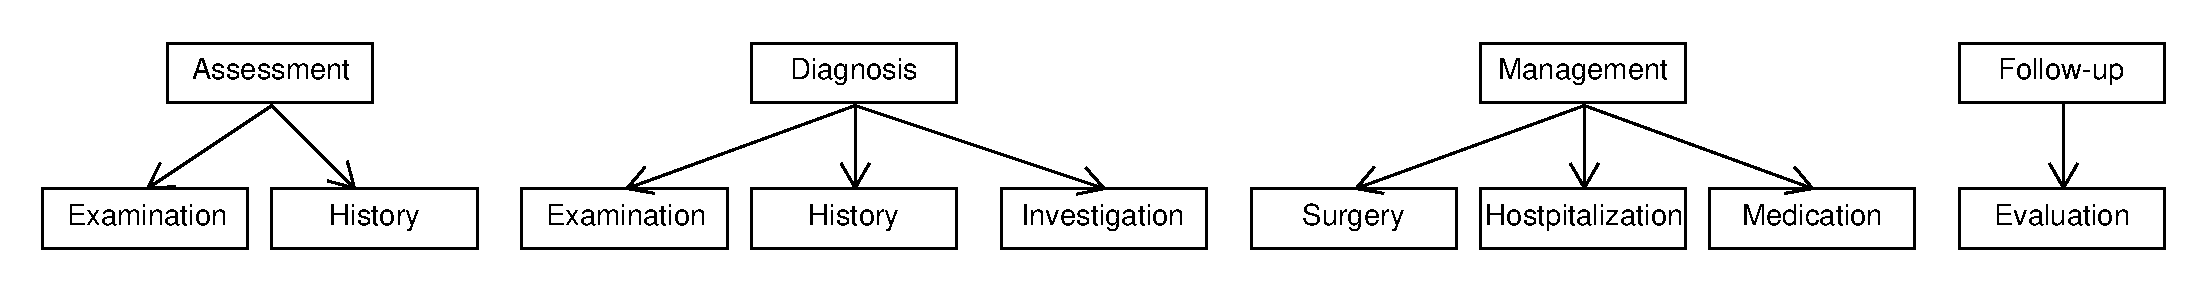
\includegraphics[scale=0.36]{KnowledgeMap2}
	\caption {By looking at the workflow- and entity models we can identify the type of questions for each content unit in the knowledge map. The content units are the parent nodes, while the leaves are the type of questions}
	\label{fig:ExpandedKnowledgeMap}
\end{figure}

As the student learns, the questions need to adapt to the student's new level of knowledge. How we do this is by defining levels, where the questions becomes more detailed at higher levels. At level 1 the questions are all about stating facts. In level 2, we create scenarios such that we follow one patient through all of the steps assessment, diagnosis, management and follow-up. The same for level 3, but the detail level will be higher. Typically the student will only be asked for categories of medication in level 2, but in level 3 the students needs to be specific about the names of the medication as well as measurements for both dosages and symptoms. See table \ref{table:ProgressionGranularity}.

\begin{table}[h!]	
	\begin{tabular}{|m{2em}|m{6em}|m{6em}|m{6em}|m{6em}|}
		\hline
		Level & Assessment & Diagnosis & Management & Follow-up \\
		\hline
		1  & Factual & Factual & Factual & - \\
		2 & Scenario & Scenario & Scenario & Scenario \\
		3 & Detailed scenario  & Detailed scenario & Detailed scenario & Detailed scenario \\
		\hline
	\end{tabular}
	\caption{The type of questions at each difficulty level}
	\label{table:ProgressionGranularity}
\end{table}




\subsection{Unlocking harder levels at a certain category}
One of the strengths with Dynamic Content Management is the focus on adaptive learning and flexible learning \parencite{Eide2008}. By adaptive learning, we mean that the student can solve problems which are suited for his knowledge level. While flexible learning means that the student can go through the learning material in the way he prefers, as long as the knowledge dependencies are met.

For the adaptability we have already covered how we progress from factual statements to scenarios and the scenarios with a higher ability to make the questions more difficult. For the flexibility we have divided the content into knowledge units: assessment, diagnosis, management and follow-up. It doesn't matter which of assessment, diagnosis and management the student finishes first.

The evaluations in each content unit has passing conditions. As an example; to complete assessment level 1, you need a score of 30 in assessment. These passing conditions are provided by the quiz author. We also recall that to unlock questions, such as management level 2, there are certain prerequisites that need to be fulfilled. In this example, all evaluations in level 1 need to be completed to unlock any level 2 questions. The flexibility is that it doesn't matter the order of level 1 evaluations the student finishes first, as long as all of them are finished.

To avoid that the student gets bored, he will not have to redo an evaluation once the passing condition is met. That means that if the student meets the passing condition of level 1 assessment and diagnosis, but not management, the student will only get questions from management level 1 the next time he takes the quiz. This makes a challenge for the scenarios. All scenario questions must be formed in a way, such that the student doesn't have to remember information from one question to another. All the necessary information should be listed in every scenario question. In that way the student won't miss important information if he completes diagnosis in a run before management and follow-up. 

Each evaluation also has a minimum required skill value. If the student gets a lower score than the required minimum skill, the evaluation gets locked and the student needs to complete the evaluation at lower level. An example is that the student plays management level 2. He completes the evaluation with a lower score than the required minimum skill. The student will have to redo management level 1 evaluation to learn the basic skills necessary to play level 2. When this situation happens, the student no longer meets the prerequisite for the other level 2 evaluations. Level 1 management needs to be completed before any level 2 evaluations can be taken. 





\section{Conversation Manager}
\subsection{Constructing scenarios and answer keys}
A quiz consists of several questions, where each question has answer keys and distractions. At level 1 these questions will be factual, and in level 2 and 3 we will work with scenarios. We write the questions in the format of a template, where we use tags to refer to variables in the entity model. The tag is a path in the entity graph. The game engine will traverse through the graph and return the value of the vertex specified by the path. The entity graph represents a patient at a certain point in the assessment or treatment. By replacing the entity graph, we can reuse the same template with different patients, generating many different questions with the same template. 

The same goes for the answer key. The answer key can be a text, one or several tags referring to variables in the entity model, or a combination of both. The application always uses the same entity graph for the scenario and the answer key. When the application traverses entity graph, the answer key and the question given always matches as they are the same patient at the same given time.

One of the problems we encountered with this method, was how to present the variables returned by the graph in a text. As an example, we can look at some of the symptoms of asthma and their type.
\begin{itemize}
	\item Wheeze is a whistling sound when you breath. In the model it is represented as a boolean. True or false. Either you have it or you don't.
	\item Age is relevant several places in the guideline. In the model it is stored as an integer.
	\item AVPU is a scale system, which clinician use to measure a patient's level of conciousness. A is alert. V, the patient is verbal which means he can somehow respond to questions. P, the patient responds to pain. The patient will react if you pinch him. U is unresponsive or unconscious. He doesn't respond to either voice or pain. The AVPU is represented in the model as an enumerate.
	\item Severity classifies the asthma severity to be either severe, model or mild. The severity is represented as a string in the model.
\end{itemize}

\begin{figure}[h!]
	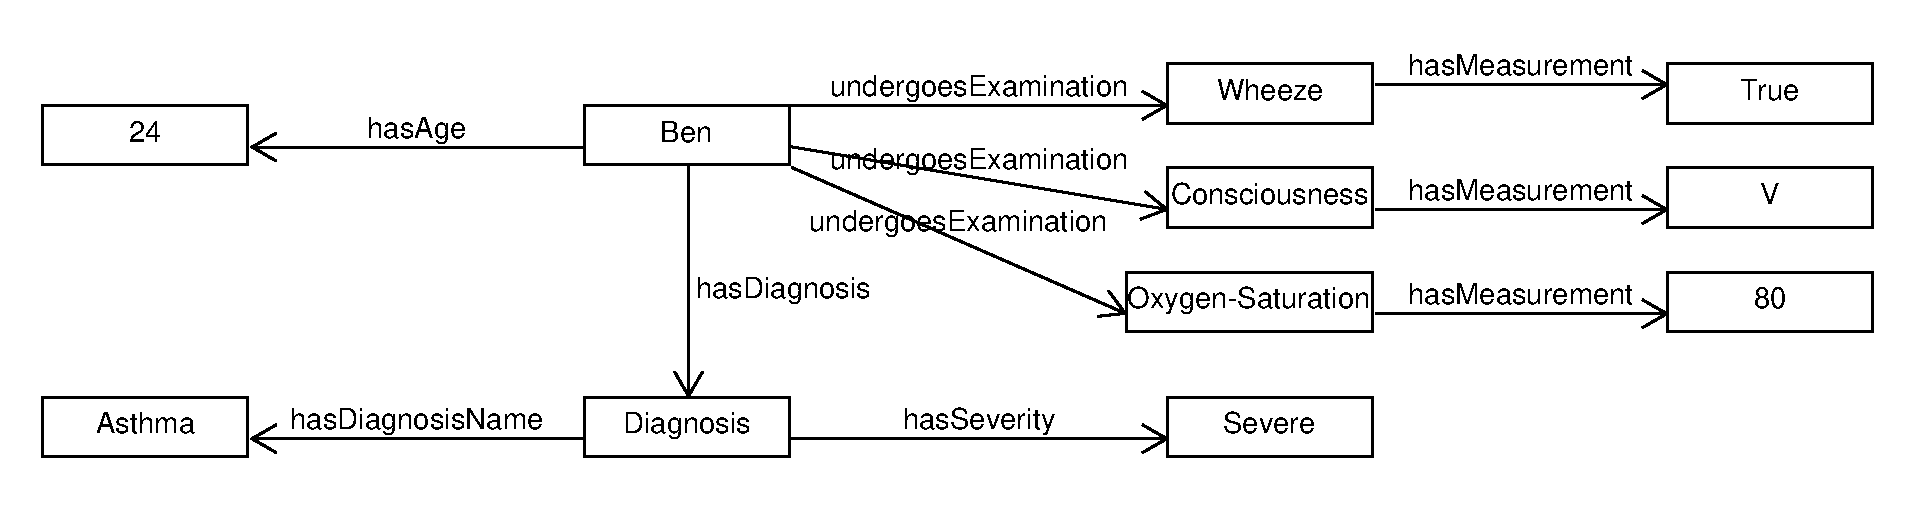
\includegraphics[scale=0.4]{EntityInstanceGraph}
	\caption {The patient object used with the template}
	\label{fig:EntityInstanceGraph}
\end{figure}

%\begin{lstlisting}[caption={My Caption},captionpos=b]
\begin{lstlisting}[caption={Question template}, frame=single, captionpos=b] 
Question:
A <%Patient.hasAge.Age%> months old patient arrives at 
the  emergency department. 
The patient has a 
<%Patient.underGoesExamination.Wheeze%>,
has conciousness level 
<%Patient.undergoesExamination.Consciousness%> 
and has an oxygen saturation of 
<%Patient.undergoesExamination.Oxygen-Saturation%>%. 
What is the asthma severity? 
\end{lstlisting}

\begin{lstlisting}[caption={Answer key template}, frame=single, captionpos=b] 
Answer key:
<%Patient.hasDiagnosis.Diagnosis.hasSeverity.Severity%>
\end{lstlisting}

This translates to 
\begin{lstlisting}[caption={Question instantiation}, frame=single, captionpos=b] 
Question:
A 24 months old patient arrives at the emergency 
department. 
The patient has a true,
has conciousness level V 
and has an oxygen saturation of 80%. 
What is the asthma severity? 
\end{lstlisting}

\begin{lstlisting}[caption={Answer key template}, frame=single, captionpos=b] 
Answer key:
Severe
\end{lstlisting}

We see that the template author needs to be aware of how the variables will be printed. Here he knows that the model will just return an integer for the oxygen saturation. He writes a descriptive text of the value first, and then adds a percentage after the variable. The severity gets nicely printed as answer key.

The problem is the boolean for wheeze, which prints a "true". It really should have printed "wheeze". We solved the presentation of consciousness in the same way as we did with oxygen saturation. However, it could be nicer to write "responds to pain", rather than just "V". When the child 12 months or older, it is often easier to read if we can present the age in years.

Another problem arrives when we replace the entity graph with another, where some of the examinations haven't been done. In traditional model driven engineering, we use something called the closed world assumption \parencite{Sadowska2019}. If a node doesn't exist, we say the value is false. But how can we say that patient doesn't have wheeze when we haven't examined? In open world assumption a none-existing vertex is "unknown" \parencite{Patel-Schneider2006} \parencite{Bergman2018}, and this strategy seems more correct for our scenario. If the vertex doesn't exist, we simply return an empty string. This further motivates us to remove the variable specific text from the template, as we don't want text representation for a variable we don't present. Example when consciousness and oxygen saturation haven't been examined:

\begin{lstlisting}[caption={Question instantiation}, frame=single, captionpos=b] 
Question:
A 24 months old patient arrives at the emergency 
department. 
The patient has a true, has conciousness level 
and has an oxygen saturation of %. 
What is the asthma severity? 
\end{lstlisting}

How we solved the problem was to add a textual presentation vertex to each of the vertices in the graph referred to by the template. If there exist a presentation for the vertex, return the presentation. If there doesn't exist a presentation, simply return the variable.

\begin{figure}[h!]
	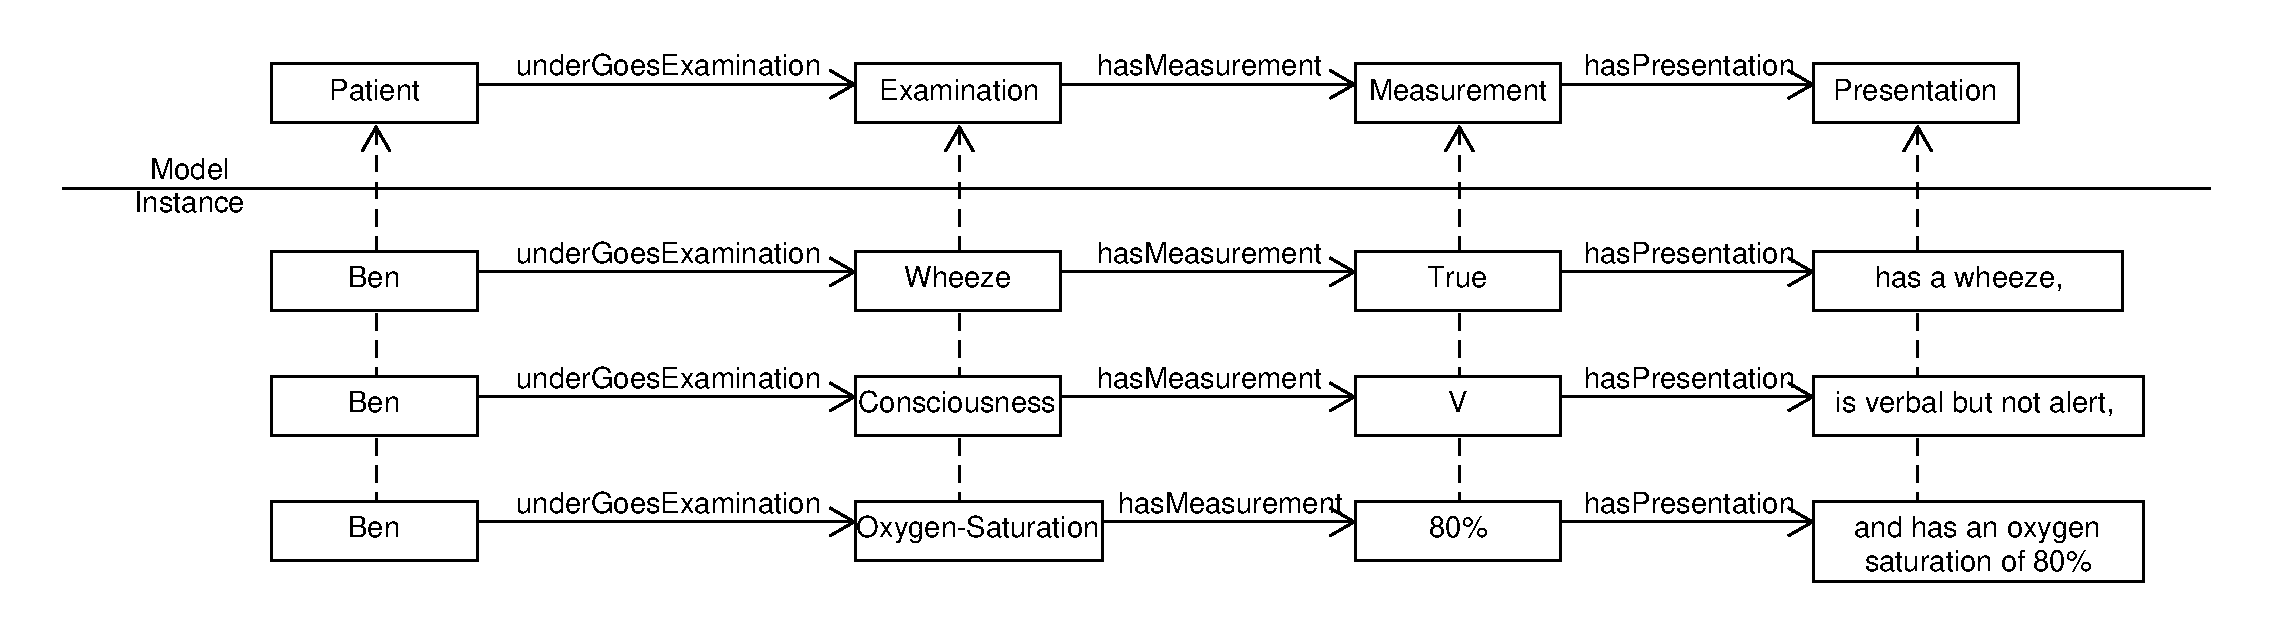
\includegraphics[scale=0.35]{GeneratingScenarios1}
	\caption {Making graph variables fit a story format}
	\label{fig:GeneratingScenarios1}
\end{figure}

\begin{figure}[h!]
	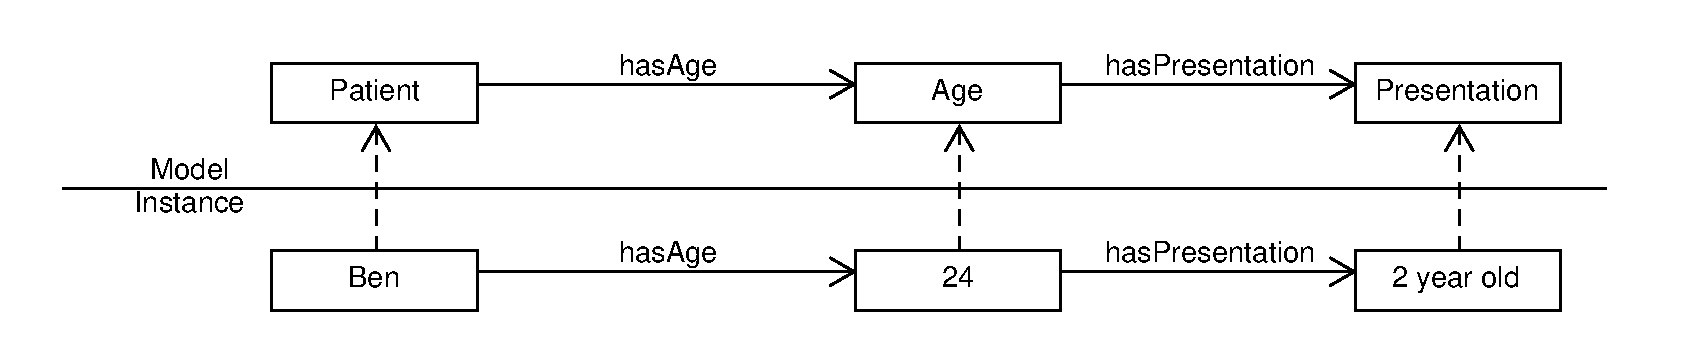
\includegraphics[scale=0.4]{GeneratingScenarios2}
	\caption {Making graph variables fit a story format}
	\label{fig:GeneratingScenarios2}
\end{figure}

\begin{lstlisting}[caption={Question template}, frame=single, captionpos=b] 
A <%Patient.hasAge.Age%> old patient arrives at 
the emergency department. 
The patient <%Patient.underGoesExamination.Wheeze%> 
<%Patient.undergoesExamination.Consciousness%> 
<%Patient.undergoesExamination.Oxygen-Saturation%>. 
What is the asthma severity? 
\end{lstlisting}

Which translates to 
\begin{lstlisting}[caption={Question instantiation}, frame=single, captionpos=b] 
A 2 year old patient arrives at the 
emergency department. 
The patient has a wheeze, is verbal but not alert 
and has an oxygen saturation of 80%. 
What is the asthma severity? 
\end{lstlisting}

This also works with the open world assumption, as a patient which haven't undergone consciousness and oxygen saturation examinations, would result in the following text:

\begin{lstlisting}[caption={Question instantiation}, frame=single, captionpos=b] 
A 2 year old patient arrives at the emergency 
department. 
The patient has a wheeze. 
What is the asthma severity? 
\end{lstlisting}

For future work, the commas and "and" should not be in the presentation vertex. This becomes a limitation where the variable can only be used in a list and has to be in a specific place in the list. The solution would be to have a list tag in the template, and have all the paths inside that tag. Then the game engine can see how many of the list items are in the graph, and can set the commas and "and" at the appropriate places.

In figure \ref{fig:IntegratedEntityGamelModels} we show how the entity-, workflow and game models work together to make a scenario. Because of limited space, we don't show the presentation vertices in the entity graph. We also combined entity graph E1 and E2 in the presentation, where E2 gets and additional medication vertex marked with red. 

\begin{figure}[h!]
	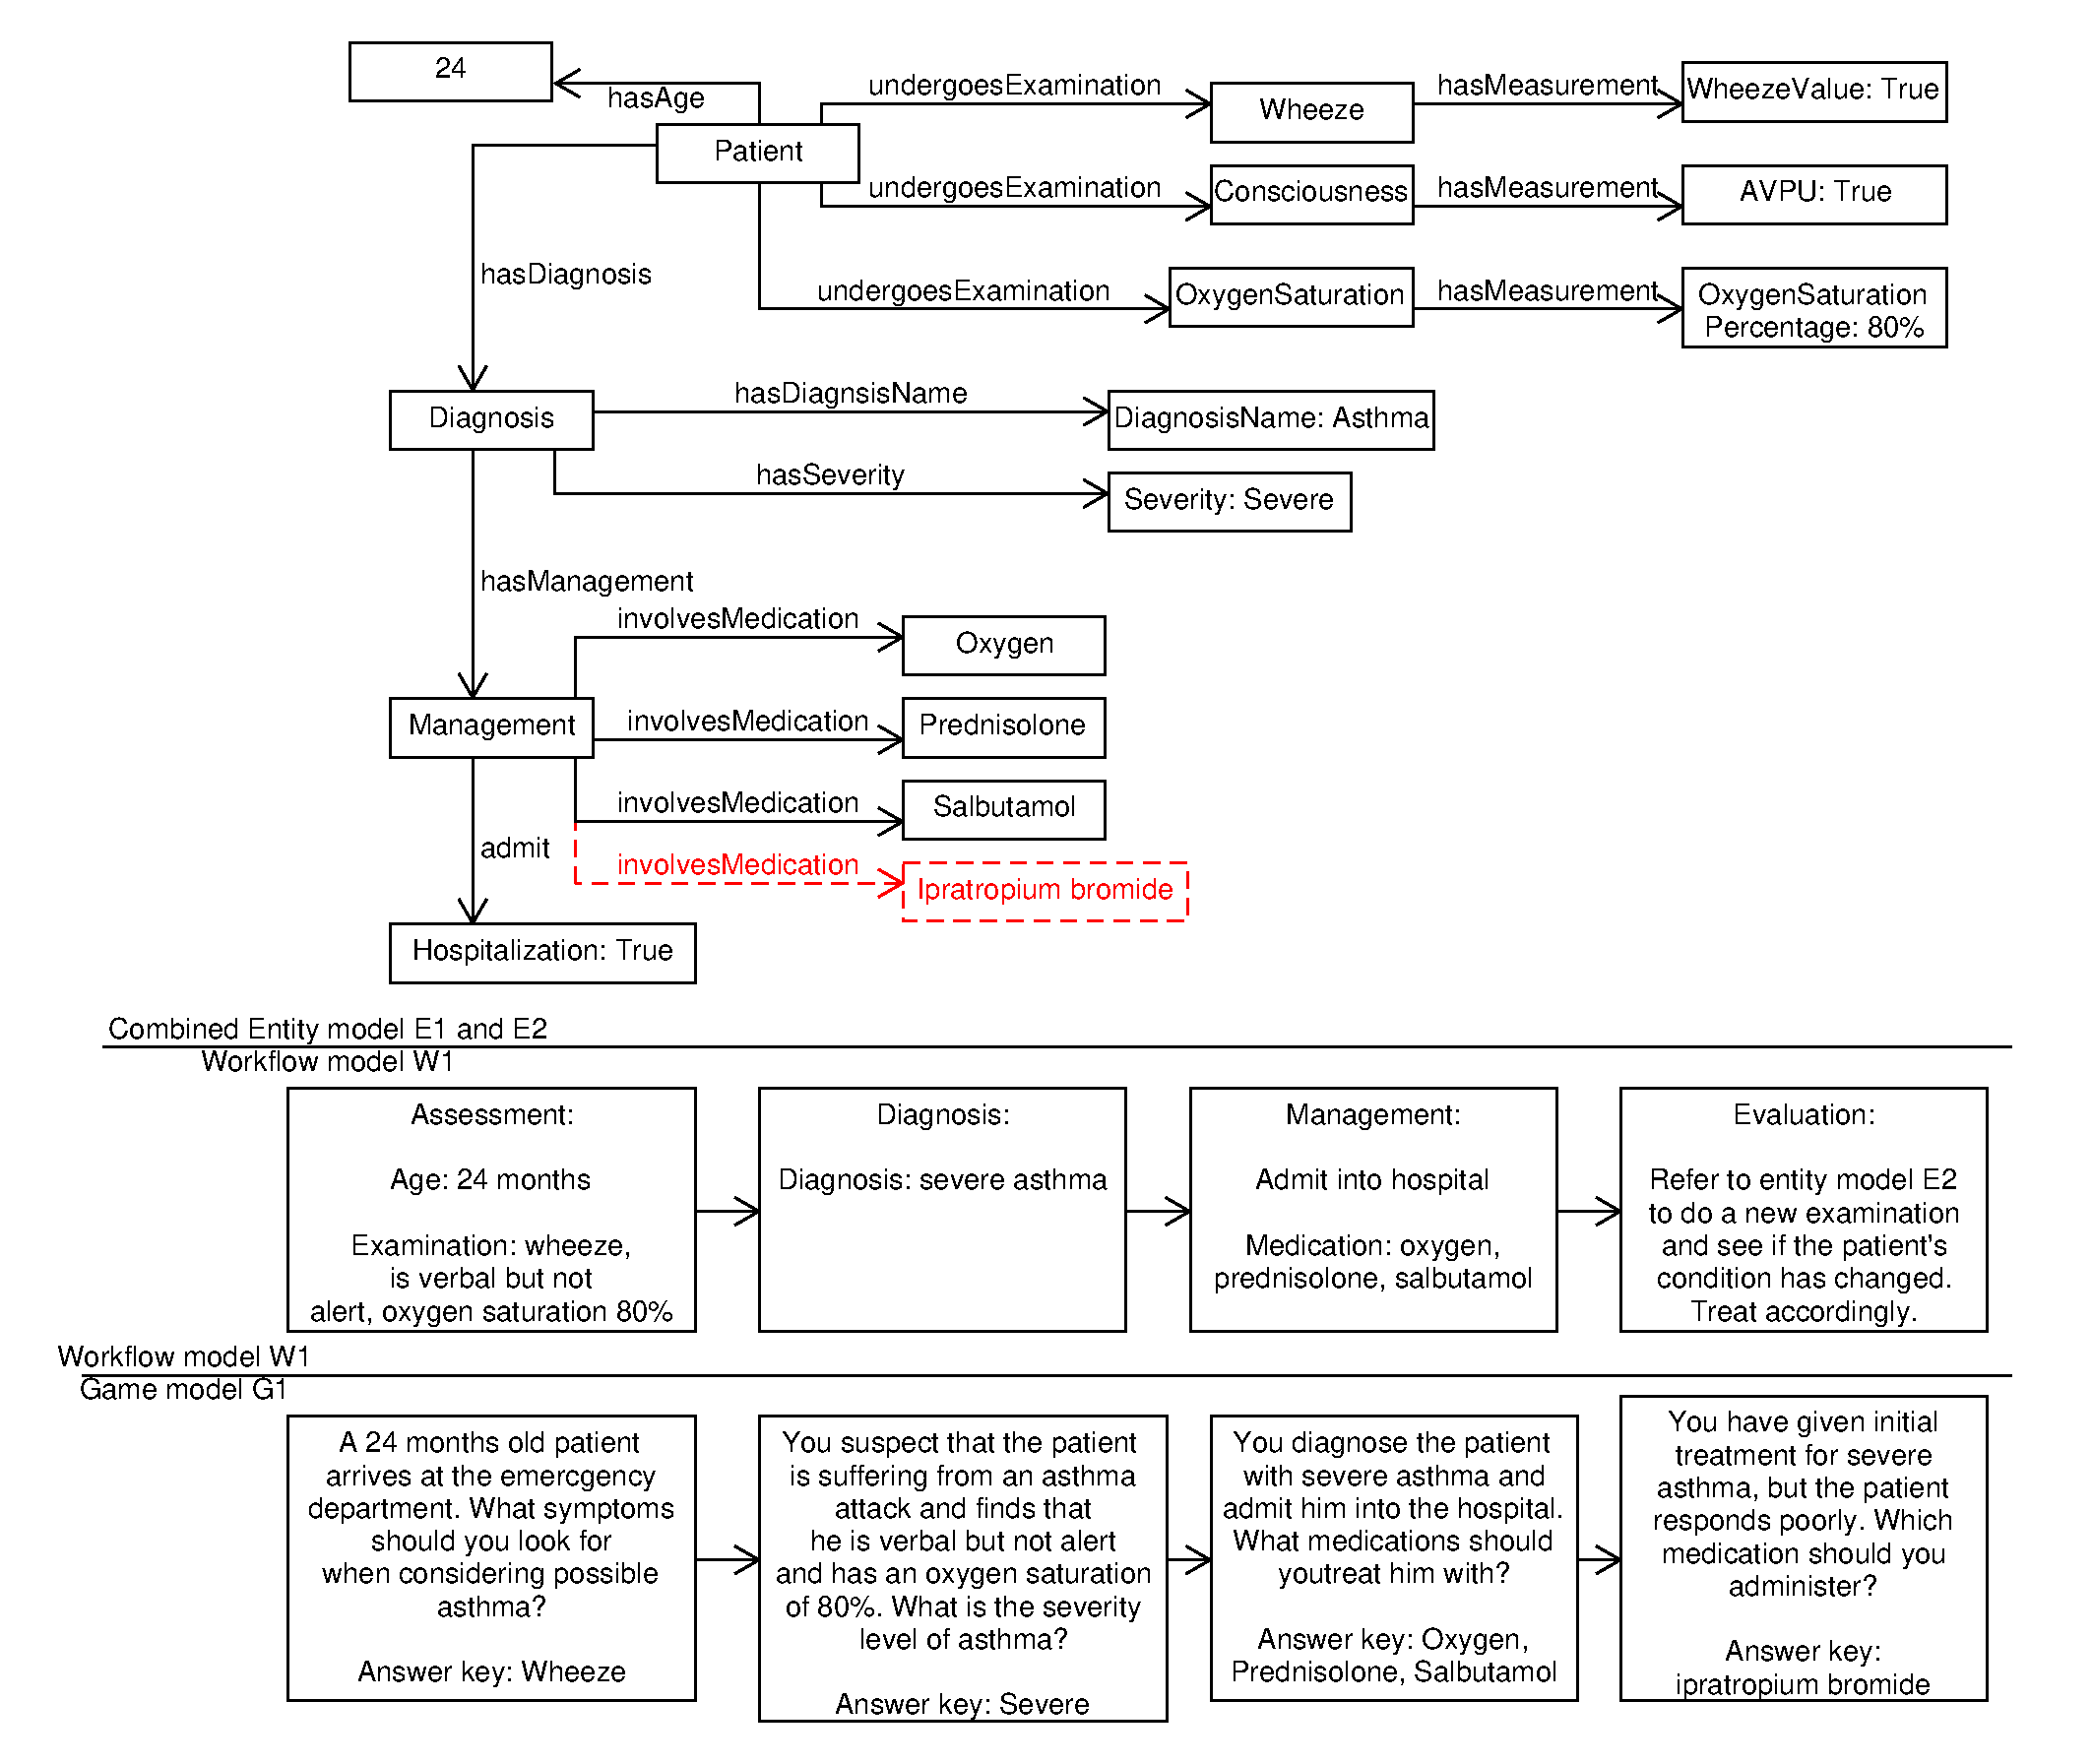
\includegraphics[scale=0.38]{IntegratedEntityGameModels}
	\caption {The entity- workflow- and game models working together to produce a scenario, taking the patient through the steps of a clinical encounter. Note that these are two entity graphs E1 and E2, where E2 gets updated with an additional red vertex Ipratopium bromide. This illustrates a patient which doesn't respond to the initial treatment, and then gets treated with ipratopium bromide}
	\label{fig:IntegratedEntityGamelModels}
\end{figure}

\subsection{Multiple-try feedback}
% https://books.google.no/books?hl=en&lr=&id=GgCPAgAAQBAJ&oi=fnd&pg=PA125&dq=Interactive+with+multiple+tries+&ots=A9Z_BJS5t2&sig=RTv1FmOzU_qic9ADjDgKdJoHamU&redir_esc=y#v=onepage&q=Interactive%20with%20multiple%20tries&f=false
% https://onlinelibrary.wiley.com/doi/full/10.1348/000709905X39134
The quiz uses a concept which is called multiple-try feedback (MTC). That means for every question the student gets more than one attempt to get the answer right. A feedback will be given immediately after each answer is submitted. The feedback consists of a message which tells whether the answer is correct or wrong. If the answer is correct, the user will receive "correct" and an explanation of the answer. If the answer is wrong, there will be no hints or explanations than just "incorrect".

\begin{table}[h!]
\begin{tabular}{ | m{7em} | m{6em}| m{5em} | m{5em} | m{5em} | } 
	\hline
	\textbf{Concept} & \textbf{Abbreviation} & \textbf{Feedback after each question} & \textbf{Multiple attempts at each question} & \textbf{Hints on wrong answer} \\ [0.5ex]
	\hline
No or delayed Feedback & NF or DF & No & No & No  \\
\hline
Knowledge of Correct Response & KCR  & Yes & No & No \\
\hline
Multiple-Try feedback with knowledge of Correct response  & MTC & Yes & Yes & No \\
\hline
Multiple-Try feedback with Hints & MTH & Yes & Yes & Yes \\
\hline
\end{tabular}
\caption{Overview over different quiz concepts}
\end{table}

The point of doing MTC, is to make the student think over what was wrong with his first answer. Did the student misinterpreter the question? Was there a detail he missed? Does the student lack the knowledge or was he just sloppy in his first attempt?

\textcite{Clariana2006} did a study where they divided 82 students into five groups. DF-, KCR, MTC and two control groups. The first control group got a text and a question at the end. The second control group got a text, but there were no question given. After 5 days,post-test was held to see what the students had learned and remembered. The post-test questions were either identical to the questions in the learning material, transposed where the order of the stem of the question and the correct-response gets reversed, paraphrased where post-test questions had the identical content as the learning material, but the phrasing was different and used different words, and a combination of transpose and paraphrasing. The results showed that DF and KCR groups performed better on identical, transposed and paraphrased-transposed questions. MTC performed better on paraphrased questions. The conclusion was that DF and KCR was much better methods for remembering the learning material word for word, but MTC was better when you have to think and reason about what you have learned.

\textcite{Attali2015} further did a did a study on NF, KCR, MTC and MTH using open ended and multiple choice questions on mathematical problems. They showed that solving an open ended question rather than multiple choice was a more efficient way to learn. The learning outcome was the same for the students using NF and KCR. However the learning transfer was greater when using multiple-try (MTC), and even more so when getting a hint on incorrect answer (MTH). They explained the results effortfull and mindful problem solving. In a multiple-try feedback, the user will have to reflect on their errors, re-evaluate the problem and understand the initial error. An open ended question will also require more effort of the student, as they have to generate a an answer rather than selecting from alternatives. On the combination of multiple-try and multiple-choice, it was suggested that some users might be less likely to review their incorrect answer and mindlessly clicking on another alternative. 



According to \textcite{Morrison1995}, students which perform badly on answer until correct questions,  will often become frustrated, loose interest for reviewing the material and probably depress learning.

% From Attali2015, students might assosiate distractions with the scenario in multiple-choice, which is counterproductive when it comes to learning.


As thinking and reasoning about a diagnosis, treatment plan, evaluation and follow-up of a treatment is part of a medical procedure, we believe that multiple-try feedback is the right approach. Because of the nature of a mobile app, where gestures are more convenient than typing sentences, multiple-choice seems to be the right choice even, though open ended questions has proven better results in. There's also a technical problem with evaluating free typed sentences.

Some of the questions in the app are too simple for a hint to be meaningful.Example: "the symptoms for asthma is" and the answer can be "cough and wheeze". Where hinting "cough", would be giving away the answer, especially in a multiple-choice format. However, the data model supports hints as links to external learning material. E.g. the student could look for the answer in the guideline itself.

We solved the "answer until correct"-problem described by \textcite{Morrison1995}, by having a "read more" button displayed upon incorrect answer. The "read more"-button will display the correct answer, an explanation and continue to the next question. Avoiding the user becoming frustrated and discouraged by having to brute-force the answer keys to progress.




\subsection{Reward system}
% SHOW ANSWER
By having multiple-try feedback, another problem rises, and that is the reward system. If there is no penalty for incorrect answers, a student which needs ten attempts per questions, will get the same score as a student which answers all the questions correctly on the first attempt.

\textcite{Attali2015} solved the problem by giving 1 point for answering correctly on the first attempt. 2/3 points for the second attempt, 1/3 for the third and 0 points if the third attempt was incorrect. A limitation with this method is that it makes no sense for the student to make more than three attempts. \textcite{Morrison1995} had another strategy where they adjust the scores by dividing the total score by the total number of attempts during the quiz. A consequence is that attempt number two will have a huge penalty which is halving the students total score. While attempt number twenty will give a very small penalty from attempt nineteen. A method to dampen this effect could be dividing the total score by the sum of reviews and number of questions. Another method could be taken the square root of the question reward for every attempt the student has on that question.

The solution we used was having a fixed value for every answer alternative. The quiz author chooses the penalty for each distraction and reward for each answer key. The idea is that the distractions can have some sort of degree of wrong or right, and this can be reflected in the scoring. On the question "what are the symptoms of asthma?", "difficulty breathing" is a more correct answer than "fever", as "difficulty breathing" is a symptom of asthma in combination with wheeze. Fever is not an asthma symptom at all. In future work, the penalties can be automated as you can see from the entity model whether the symptom belongs to the asthma guideline or not. A distraction from respiratory disorders may give a larger penalty than a distraction from the asthma guideline, but smaller penalty than symptoms not belonging to respiratory diseases.

Both \textcite{Attali2015} and \textcite{Morrison1995} avoids the scenario where the user gets a total minus score. This may be a strength of these methods, as a negative total score seems like a very harsh feedback and might demotivate the student. In our solution we use negative numbers as penalties on distractions, such that a negative total score may happen. We try to limit the likelihood of a negative score by providing a very high reward for a correct answer and a very small penalty for a distraction. Typically the reward is 10 points and the penalty -1 og -2 points. The intention is to encourage the student to review the incorrect answer and try again. As the format is multiple-choice and the penalty-reward ratio, there is a little risk involved trying multiple times. But giving up by clicking "learn more", the student will not get an additional penalty, but will miss out on the reward. By clicking answer alternatives mindlessly and consequently clicking "learn more" will probably not end up in a negative score, but is more likely to end up in a negative score than mindlessly click answer alternatives until correct.

%----------------------------------------------------------------------------------


%Each question will have several answer alternatives the student can choose from. Each answer alternative will have a reward or penalty related to them. The correct answer will have a great reward, while wrong answers will have a small penalty. The quiz author will have the opportunity to specify the rewards, such that he can give even smaller penalties for partly correct answers. The idea of the reward- penalty system is to increase learning. if the student answers wrong the first time, he will be given the possibility to reflect over the question once more or perhaps read the guideline to learn before he commits his second attempt. We are aware that providing a minus score for making an attempt can be very demotivating, but it is to avoid the situation where a student gets the same (or better) score for making ten attempts than only needing one attempt. A small penalty will have a very small impact when the reward per question is high, but in situations where the student performs very poorly and ends with a negative total score, it is possible to adjust this to a small positive score on presentation for the student. Not giving a too harsh feedback for trying to learn.



%\textcolor{red}{A solution to having a not very strict game, encouraging to playing and learning, one can also have a very strict examination version. The idea is that after examination, the results will be sent to the lecturer (or a governing body of some kind) to evaluate what the overall knowledge of the students, as well as details of what the students are really good in and where do they struggle. The lecturer can then target the weak of points of the students in one of the next lectures. }




\section{User manager}
The user manager stores the scores of previously played quizzes on the student's game. By fetching the last played game for a specific quiz, it knows the student's current knowledge level. The stored scores represents the student map, and also shows the student's current position in the learning map. By analyzing the student map, we can see the student's progressions.

The user manager will also keep track of the scores during a quiz game. At the end of the game, the user can be notified if he got demoted to an easier level, promoted to play more difficult content or show the student how close he is to complete the current difficulty level.

\subsection{Visualization of game statistics}
The student needs some feedback, where he is in the learning map, how close he is to pass an evaluation, how close he is to progress to the next level and in the case where he gets relegated to an easier difficulty level.

The scores for the evaluations can be shown as bars in a graph, and the passing conditions as a line. When the bars reaches or passes the line, the student knows that the he has met the passing condition for the evaluation at that level. This can also work as a motivation for the student, as he sees that he gets closer and closer to the passing condition as he learns he more and performs better.

To visualizing where the student is in the learning map, has been solved by showing the learning map in almost a table format. Colour combinations shows which evaluations have been unlocked, which are locked and which are the current ones the student plays. Red and green indicates whether a student gets relegated from a level or whether he progresses to the next level.


\section{Conceptual model of how all the classes are connected in Game Engine}
The conceptual model of the game engine is shown in figure \ref{fig:ConceptualGameElements}. Category is a quiz game for a certain CPG, such as the paediatric possible asthma guideline \parencite{RepublicofKeny2016}. Each of these quiz categories are divided into several disciplines. Disciplines are themes in knowledge units, which we identified using DCM (dynamic content management). Each of these knowledge units contain evaluations at different difficulty levels. These evaluations are collections of questions, which contain a collection of multiple choice questions and answer elements.

The quiz data are read from JSON-files, which are produced by a content author. The quiz author defines a quiz for a specific CPG. He identifies themes for content units, which contains evaluations with varying difficulty levels. The questions are written in a template format, which we have already covered. The templates contain tags, which refer to vertices in the entity graph, representing a given patient. The answer key is also such a tag, referring to one or more vertices in the entity graph. When the quiz is initialized, the tags will be replaced with values from the entity graph. The content author will write answer alternatives for each question, where he specifies a reward (or penalty) for each of the answer alternatives. An answer alternative which matches the answer key value in the entity graph will represent the correct answer. The content author needs to know what is in the entity graph to be able to provide meaningful rewards.

The student skills is the scores from the last played game, and is fetched from the database on the student's phone. The allowed- and unallowed levels are calculated from the student skills and the requiredMinSkill for each level. Unallowed levels are levels that the student can't play and are locked for the student, as the student's score is lower than the required minimum skill.

A new instance of skill will be created when the student starts a new game. This instance will hold the scores for the current game, and will be stored to the phone's database once the game has been completed. This score determines which levels the student can play in the next game of this category.


\begin{figure}[h!]
	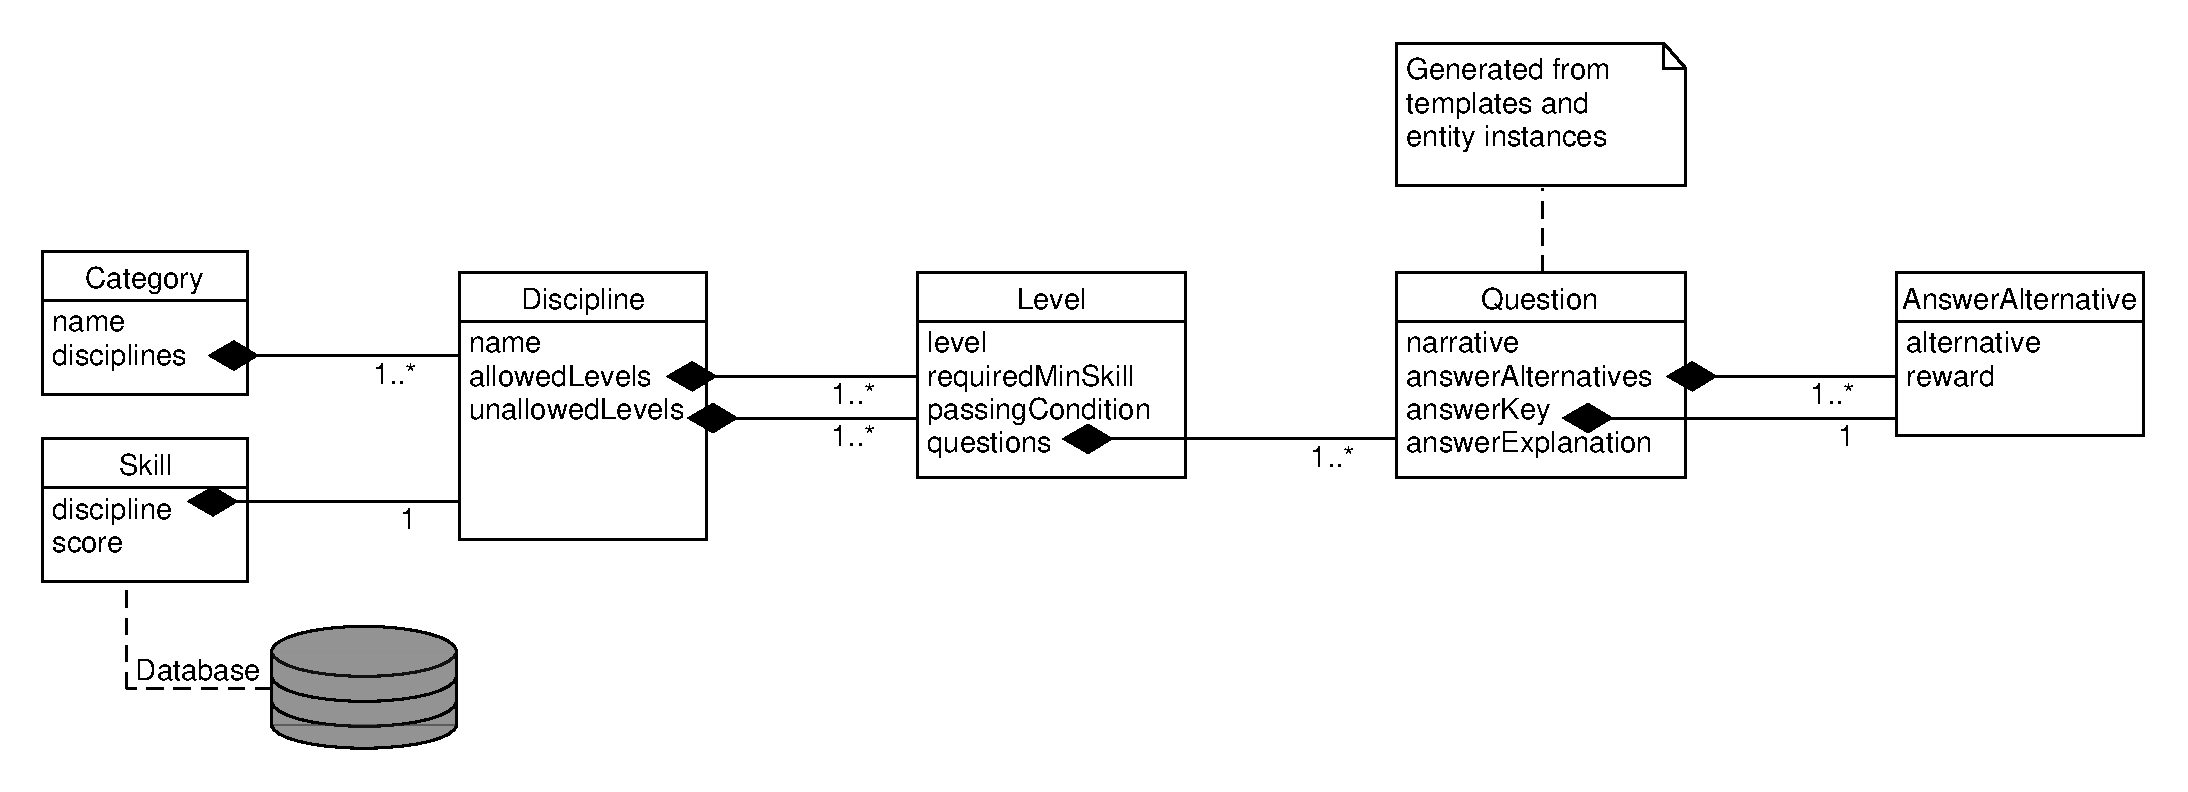
\includegraphics[scale=0.36]{ConceptualModelGameElements}
	\caption {Conceptual model for the game elements}
	\label{fig:ConceptualGameElements}
\end{figure}

One problem with the conceptual model is that it is somewhat complex. Once we have determined which levels we should pick questions from and we have generated the questions, we really don't need the structure. Especially when playing scenarios, it is nice to just go through an ordered array, instead of dealing with "now I've played the third question of level 2 diagnosis, the next question in this scenario is the third question in level 2 management, unless I've already completed level 2 management in the previous run of the game. Then the next question is follow-up instead". We rather deal with the problem at the initialization phase and just go through the array when playing the game. A solutions is to implement the façade pattern \parencite{Gamma1994}, such that other parts of the system can use the game engine, without having to deal with the underlying complexity. 

% Not sure whether this is facade or mediator pattern thouh

\begin{figure}[h!]
	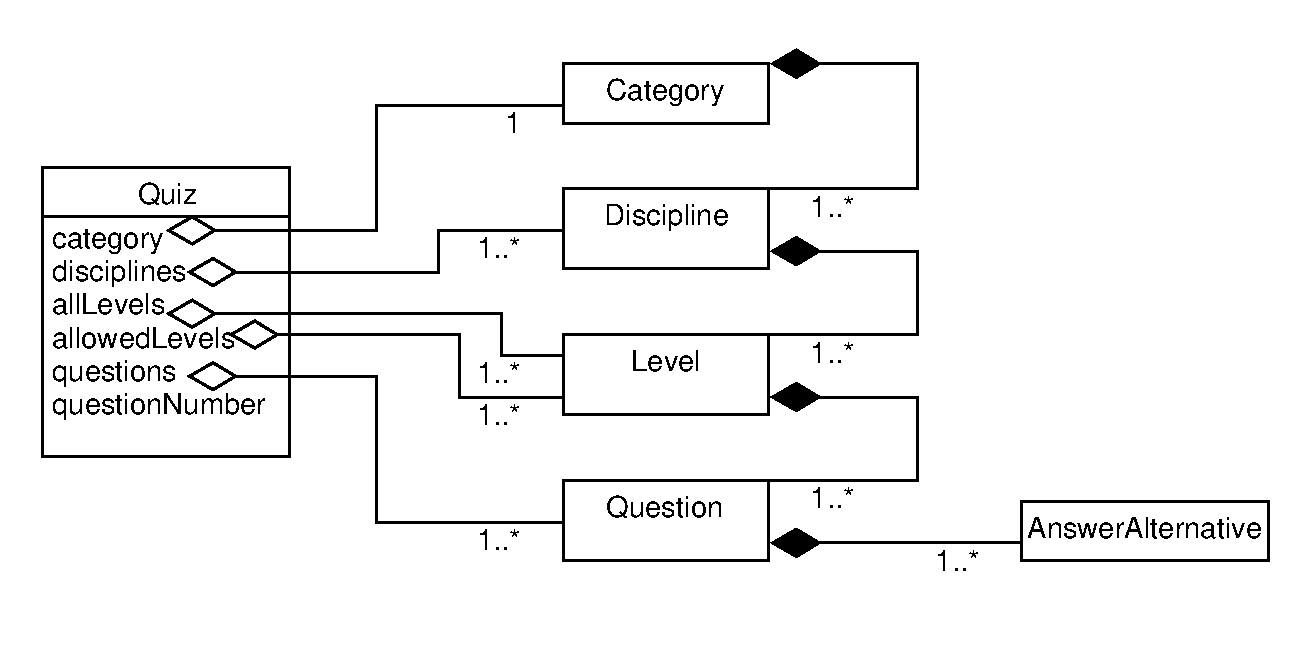
\includegraphics[scale=0.4]{GameEngineFacadePattern}
	\caption {Façade pattern hides the complexity of the game engine and makes it easier for other parts of the system to use it}
	\label{fig:GameEngineFacadePattern}
\end{figure}

%\textcolor{red}{Should I show how I populate the models with data from JSON and database? I'm not very happy about the code on that part.}
% DON'T KNOW IF I SHOULD SHOW THE GAME ENGINE PACKAGE HOW TO POPULATE THE MODELS AS THIS CONTAINS HARDCODED AND NASTY STUFF TO GET PROGRESS QUIKLY

%\begin{itemize}
%	\item DAO
%	\item Models
%	\item Templates/Narratives/AnswerKey
%	\item Quiz is kind of an interface
%\end{itemize}




 

\section{Summary}
The chapter is structured after the conceptual training managers in the game engine. Question flow manager, conversation manager and the user manager.

The question flow manager uses the Dynamic Content Manager (DCM) to make the questions adaptable to the student's knowledge level and flexible such that the student can choose his own path through the learning content. We used the workflow model as a base, to categorize the learning material, and we identified knowledge dependencies between them, making a knowledge map. We saw how we could make three difficulty levels by adjusting the detail level of the questions, by going from factual questions, to scenarios and then detailed scenarios. 

The conversation manager made textual questions by using instances of the entity model and templates. Tags in the template pointed to vertices in the entity model, such that we could produce many questions with one template, pairing it with different instances of the entity model. However, the entity model had to be expanded with presentation vertices as the data types couldn't be directly parsed into a textual presentation. 

Further we argued why we wanted to use multiple-try questions with feedback. The student can try as many times as he wants to get the answer correct. The idea is that the student has to revise the question and reflect on why the question was wrong and how can he correct it. We also described the reward system, which will fit the multiple-try approach. A student with ten attempts should get a lower score than a student which answers correctly on the first attempt.

We then described a conceptual and technical model of how all the classes are connected in the game engine.



